\documentclass[%
 reprint,
%superscriptaddress,
%groupedaddress,
%unsortedaddress,
%runinaddress,
%frontmatterverbose, 
%preprint,
%showpacs,preprintnumbers,
%nofootinbib,
%nobibnotes,
%bibnotes,
 amsmath,amssymb,
 aps,
 pra,
%prb,
%rmp,
%prstab,
%prstper,
%floatfix,
]{revtex4-1}

\usepackage{graphicx}% Include figure files
\usepackage{dcolumn}% Align table columns on decimal point
%\usepackage{bm}% bold math
\usepackage{fullpage}
\usepackage{epsfig}
\usepackage{amsmath}
\usepackage{amsfonts}
\usepackage{amssymb}
\usepackage{float}
\usepackage{pstricks}
\usepackage{cancel}
\usepackage{lipsum}
%\usepackage[nottoc,numbib]{tocbibind} %Uncomment for bibliography to be its own numbered section
\usepackage{units}
\usepackage{listings}
\usepackage{xfrac}

\graphicspath{{./plots/}}

\begin{document}

\preprint{APS/123-QED}

\title{\textbf{Lab Report: X-Ray Diffraction and Florescence} \\ \small{An Investigation of Characteristic Transitions of Atoms}}
\author{Joshua LaBounty}
\author{Thomas Krahulik}
\affiliation{Stony Brook University --- PHY 445}

\date{\today}

\begin{abstract}
	In this experiment, we investigate the characteristic x-rays produced by atomic transitions of various elements, according to Moseley's Law.
\end{abstract}
\maketitle

\section{Introduction}

\section{Review of Previous Work}

\section{Experimental Setup}

\subsection{X-Ray Florescence}

\begin{figure}[H]
	\centering
	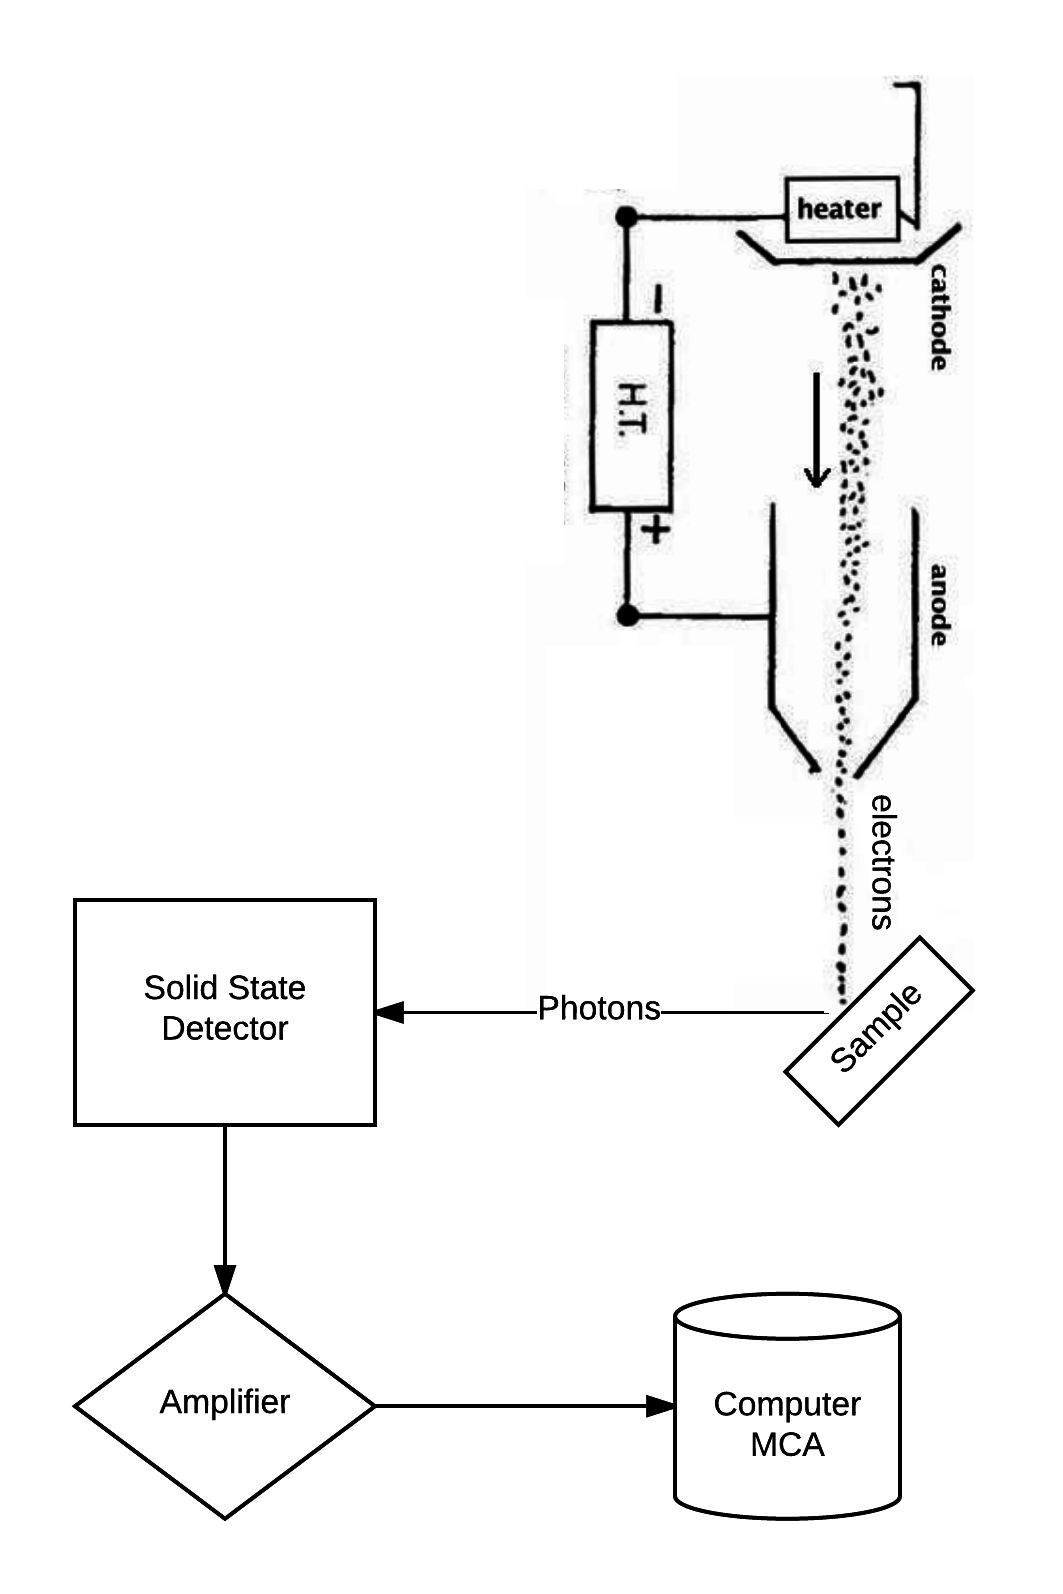
\includegraphics[width=0.25\textwidth]{xrf_experiment.png}
	\caption{Experimental Setup used in XRF portion of the experiment.}
	\label{fig:xrf_setup}
\end{figure}

The apparatus used in our measurements of x-ray florescence consists primarily of two components, an electron gun and a solid state detector, as shown in Figure \ref{fig:xrf_setup}. The electron gun operates by running a current through a filament, typically made out of tungsten due to its resilience to high temperatures, in a potential. Electrons are 'boiled off' the filament (a process known as thermionic emission) and are accelerated towards the anode. Some of the electrons strike the anode, but the rest escape through the opening into a collimated beam of particles. The energy of these electrons is defined by their accelerating voltage: $E_{e^-} = qV$, while their number is defined by the current.  These electrons impact the sample and cause it to emit photons, which are then picked up by the detector. The detector is a Silicon p-i-n diode manufactured by Amptek. Photons which are incident on the detector are first met with a window made of Beryllium, which is opaque to photons whose energies are below $\approx ~1~keV$. Photons whose energies are high enough to pass through this window then deposit their energy in the sensitive volume of the detector, ionizing the silicon atoms and creating a number of electron-hole pairs in the lattice structure. A bias voltage across the diode causes these electron/holes to flow and be read into the detector as a pulse of charge, whose magnitude is directly proportional to the energy which was deposited in the detector by the photons. This pulse is passed through an amplifier, which is then passed into the multi-channel analyzer (MCA), and then from there into the computer system. From there, the information is saved in a format which can be read into our data analysis software, ROOT. This software is developed and maintained by scientists at CERN, and contains many useful fitting and histogram manipulation packages. We also performed independent cross checks of its $\chi^2$ minimization techniques, which can be found in Appendix \ref{section:root}.

\subsection{X-Ray Diffraction}

\begin{figure}[H]
	\centering
	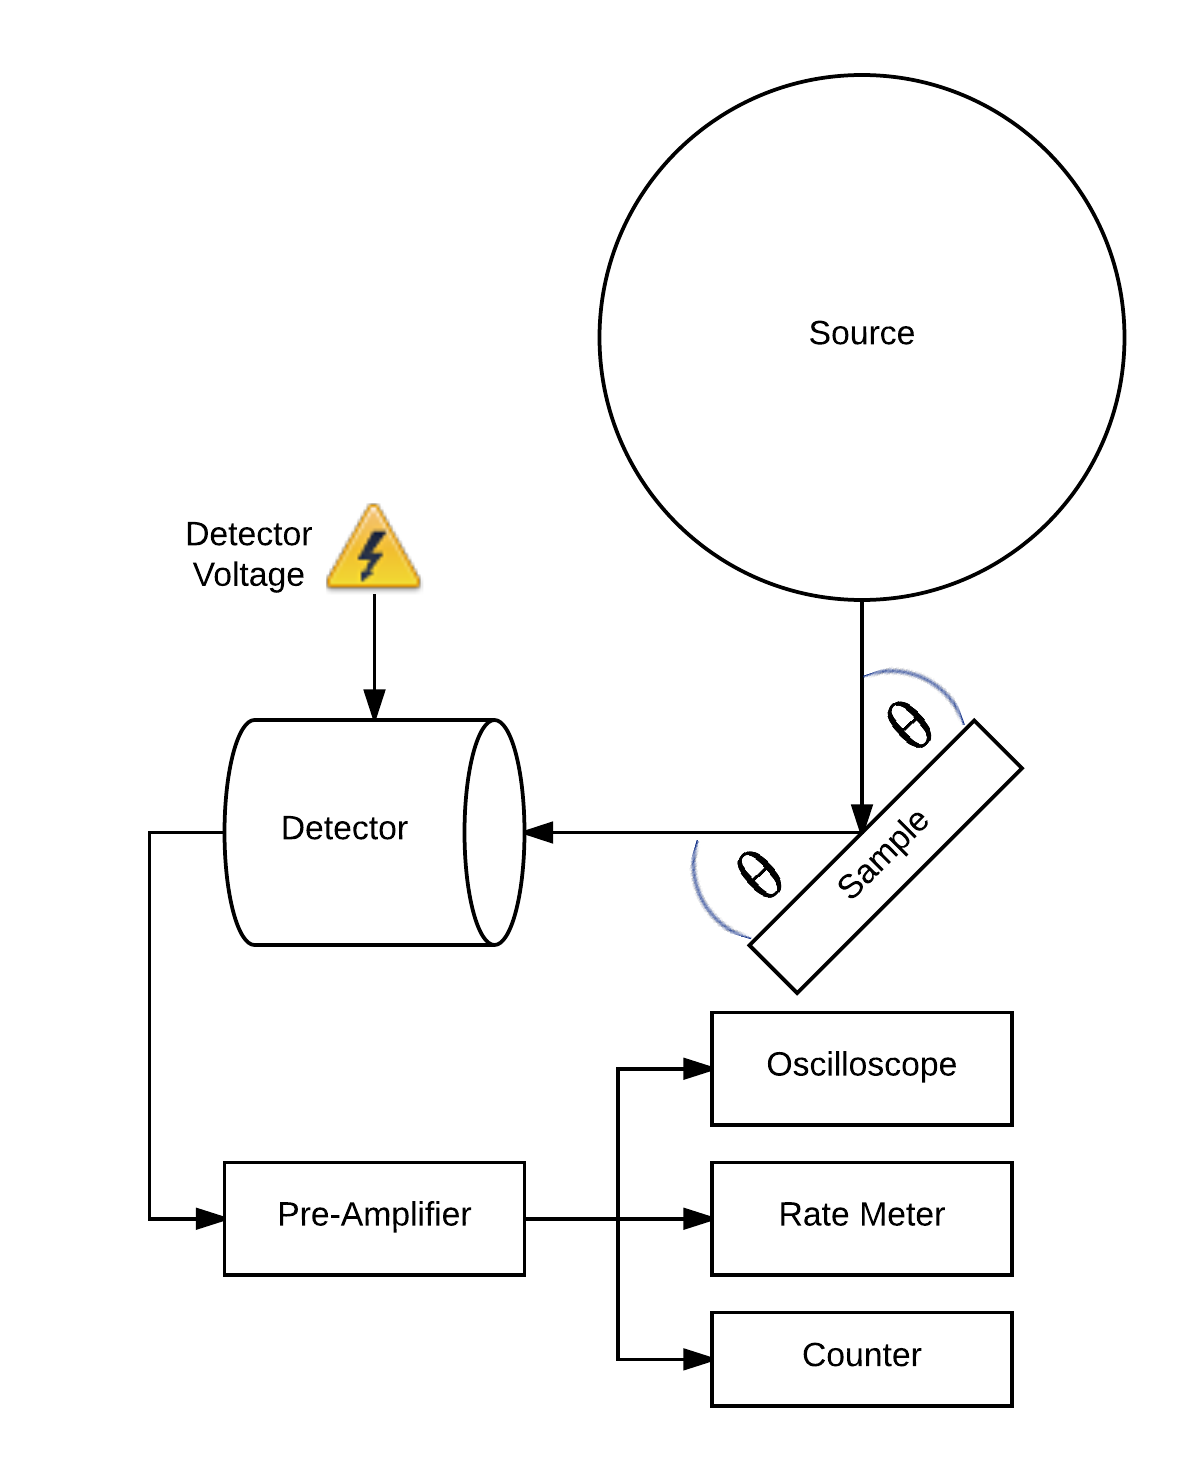
\includegraphics[width=0.3\textwidth]{xrd_experiment.png}
	\caption{Experimental Setup used in XRD portion of the experiment.}
	\label{fig:xrd_setup}
\end{figure}

This experiment consists of three primary components: the x-ray source, the goniometer, and the detector. The x-ray source uses the same method of x-ray production as the setup detailed above. However, instead of switching the samples out to change the characteristic x-rays of the system, here the target sample for the electrons is kept constant, and is composed of copper. This means that the characteristic x-rays we expect to see are those produced by copper: $K_\alpha = 8037.8 ~eV= 0.154358 ~nm$ and $K_\beta = 8905.29 ~eV = 0.139322 ~nm$. These x-rays are collimated by sheets of lead with small openings and then allowed to stream freely towards the sample. The second portion of the experiment is the goniometer, which keeps the relative angle of the sample and the detector constant: $\theta_{\text{detector}} = 2\theta_{\text{sample}}$ (relative to $\theta = 0$ defined by the path of the undiffracted x-rays). The x-rays which are diffracted off of the sample then enter the detector. This detector differs from the previous version in that it is a Geiger-Muller detector. 

In this detector, a low-pressure inert gas is encased in a cavity. At either end of this cavity is an anode and a cathode, across which a high voltage is applied. When ionizing radiation enters the cavity, molecules of the gas become ionized. The electron and nucleus then fly in opposite directions, accelerates towards the anode and cathode respectively. The ionized atom, being much more massive than the liberated electron, travels a much shorter distance, and thus stays relatively close to its original position.  As the electron travels through the gas, it causes the ionization of subsequent electrons in an 'avalanche', effectively multiplying its own signal. This flow of liberates electrons creates a fast pulse of charge which is read by the tube as a single event. After the pulse is complete, the atoms in the gas return to their neutral state and the detector is ready to detect another event. The time that the pulse takes is known as the \textit{dead time} of the detector, as events can only be detected one at a time, and the detector is 'dead' to the world until the initial pulse is completed. 

This pulse of current is sent into a pre-amplification system, to increase its magnitude to levels which are more detectable, and from there into a counter, rate meter, and oscilloscope. The oscilloscope serves only to show a visual representation of the pulses, and we will use this output later to characterize the dead time of our detector. The rate meter gives us a measure of the counts/second the detector is seeing, and warns if the detector is becoming saturated (i.e. events are coming in too quickly to all be counted). The counter simply records the number of events in a specified amount of time. We will compare the output from the counter across a wide range of angles in order to determine the number flux of photons at each angle. We recorded this data manually and input it into an excel spreadsheet, so it could be plotted in real time. In order to perform our final analysis, this spreadsheet was converted into a \verb|.txt| file which we then read in to ROOT.

\section{Measurements}

\subsection{X-Ray Florescence}

\subsubsection{Characterization of the Detector}

Before performing an analysis of x-ray fluorescence, we had to calibrate the energy scale of the MCA to determine the conversion between the channel number ($n$) of a detected photon and its energy. In order to perform this calibration, x-ray fluorescence spectra were collected for various samples with known energy peaks. Fig.~\ref{Fig:InXRFSpec} displays an example spectrum with fitted peaks.

\begin{figure}[H]
	\centering
	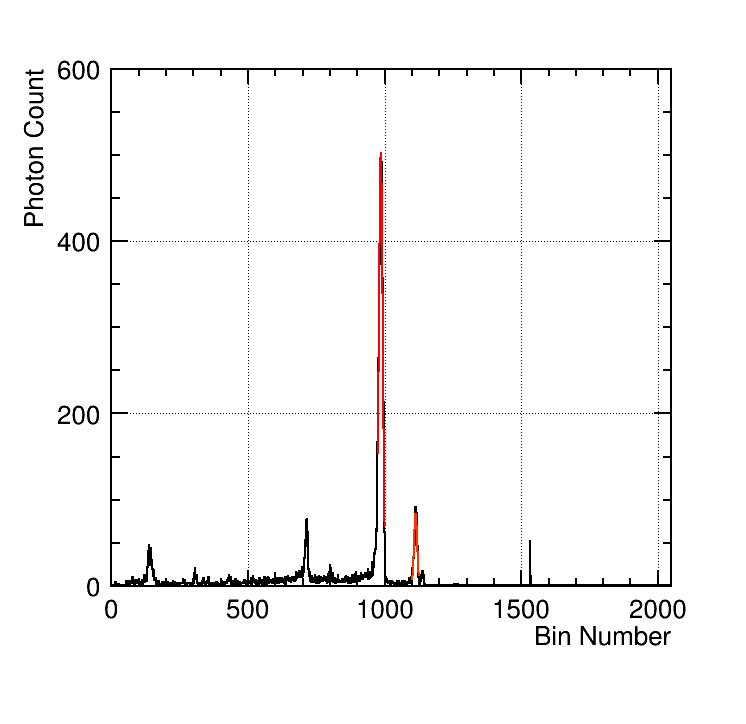
\includegraphics[width=0.45\textwidth]{InBinnedSpectrum.png}
	\caption{X-Ray Fluorescence Spectrum for Indium}
	\label{Fig:InXRFSpec}
\end{figure}

Each peak on one of these spectra was fit with a Gaussian distribution to find the mean value of the peak. This mean value was stored as the bin number corresponding to the peak of known energy provided by external sources. We collected corresponding energies and bin numbers for several samples of different elements to generate the energy vs bin number plot in Fig.~\ref{Fig:Evsbin}.

\begin{figure}[H]
	\centering
	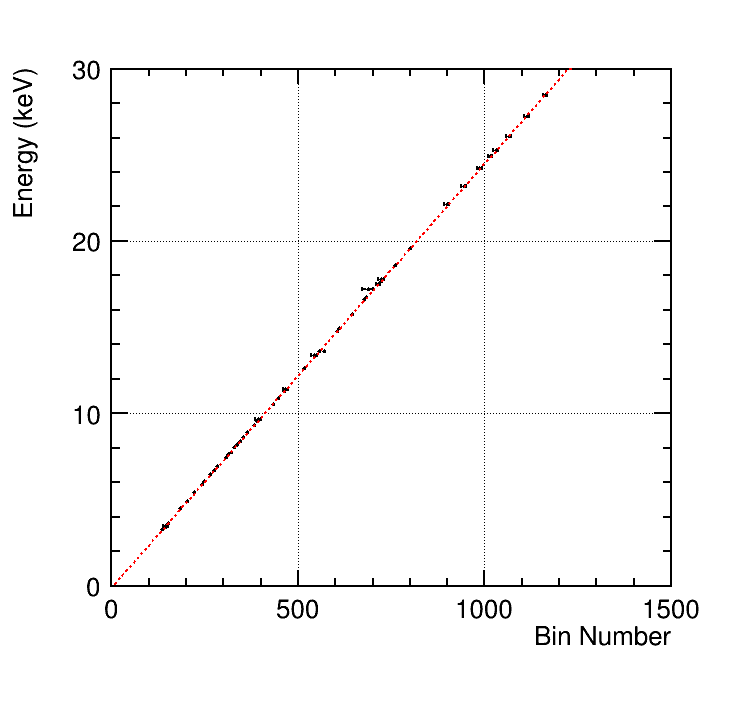
\includegraphics[width=0.45\textwidth]{EvsBin.png}
	\caption{Energy vs Channel Number Calibration Plot}
	\label{Fig:Evsbin}
\end{figure}

The linear fit on this plot provided us with the energy calibration in Eq.~\ref{eq:ECalib}.
\begin{gather}\label{eq:ECalib}
E = 0.0245644n - 0.0545754
\end{gather}

With this calibration, we could then calculate the energies of peaks in our x-ray fluorescence spectra. As previously discussed, peaks in the energy spectra for different elements were fit with a Gaussian distribution to find the mean value of the peaks which we converted to energy using our calibration. Each energy peak we analyzed corresponded to the $K_{\alpha}$, $K_{\beta}$, etc. transitions which we could confirm with outside sources. For each type of transition, we could record the atomic number, $Z$ and the energy of the emitted x-ray photon for several samples. For a more clear analysis of Moseley's Law, we derived Eq.~\ref{} in the following manner to obtain the linear relationship expressed in Eq.~\ref{Eq:MLawLinear}.

\begin{align*}
A(Z - \sigma)^{2} &= E\\
A(Z - \sigma)^{2} &= h \nu\\
Z - \sigma &= \sqrt{\frac{h}{A}}\sqrt{\nu}
\end{align*}
\begin{equation}\label{Eq:MLawLinear}
Z = \sqrt{\frac{h}{A}}\sqrt{\nu} + \sigma
\end{equation}

As demonstrated by Eq.~\ref{Eq:MLawLinear}, plotting data of $Z$ vs. $\sqrt{\nu}$ should yield a linear relationship with a slope of $\sqrt{\frac{h}{A}}$ and an offset equal to the screening parameter $\sigma$. We performed this analysis for many samples of different elements to generate the plot in Fig.~\ref{Fig:MLawPlot}.

\begin{figure}[H]
	\centering
	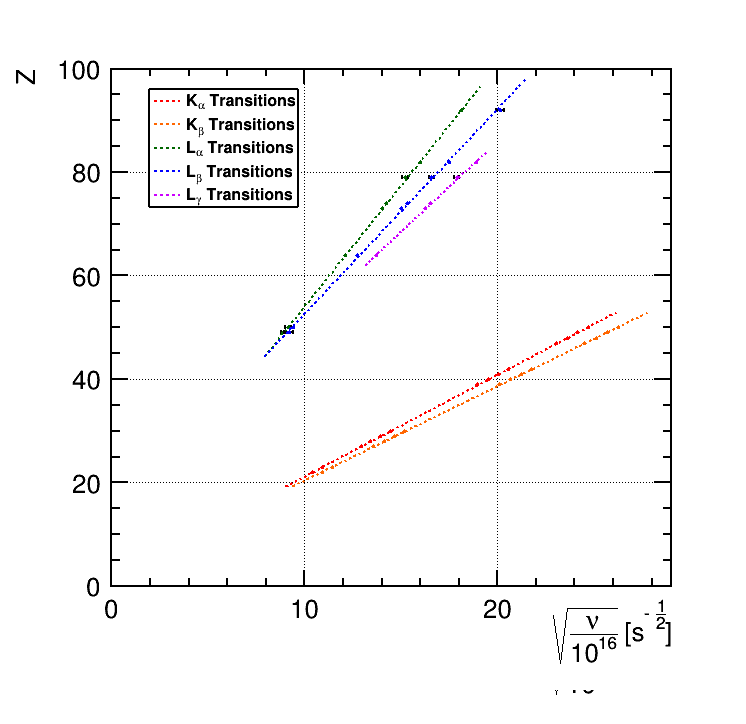
\includegraphics[width=0.48\textwidth]{MoseleyLawPlot.png}
	\caption{Plot Displaying Moseley's Law for $K_{\alpha}$, $K_{\beta}$, $L_{\alpha}$, $L_{\beta}$, and $L_{\gamma}$ Transitions}
	\label{Fig:MLawPlot}
\end{figure} 

\begin{table}[htbp]
	\begin{center}
		\begin{tabular}{|c|c|c|c|}
			\hline Transition & $\sqrt{\frac{h}{A}}$ ($ 10^{-8} s^{\frac{1}{2}}$)  & $A$ ($10^{-18} J$) & $\sigma$ \\
			\hline $K_{\alpha}$ & $1.964 \pm 0.009$ & $1.717 \pm 0.016$ & $1.621 \pm 0.166$ \\
			\hline $K_{\beta}$ & $1.824 \pm 0.007$ & $1.991 \pm 0.015$ & $2.240 \pm 0.141$ \\
			\hline $L_{\alpha}$ & $4.668 \pm 0.056$ & $0.304 \pm 0.007$ & $7.470 \pm 0.814$ \\
			\hline $L_{\beta}$ & $3.959 \pm 0.051$ & $0.423 \pm 0.011$ & $13.126 \pm 0.754$ \\
			\hline $L_{\gamma}$ & $3.491 \pm 0.074$ & $0.544 \pm 0.023$ & $16.215 \pm 1.235$ \\
			\hline
			
		\end{tabular}
	\end{center}
	\caption{Calculated Parameters in Moseley's Law for Each Type of Shell Transition}
	\label{Tab:XSecCompare}
\end{table}

\subsection{X-Ray Diffraction}

\subsubsection{Characterization of the Detector}

To begin this experiment, we needed to characterize the behavior of the detector with respect to each one of the variables.

\subsubsection{Determination of the Dead Time}

\begin{figure}[H]
	\centering
	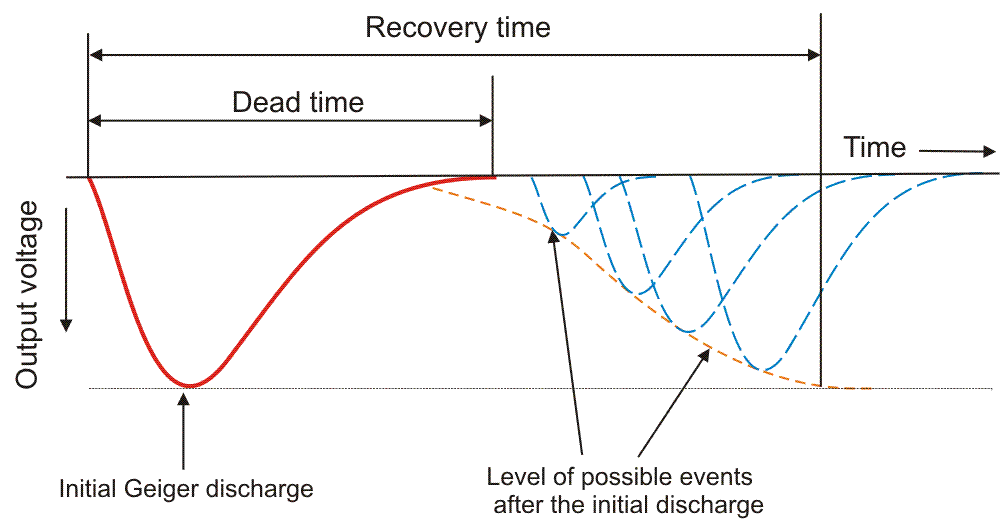
\includegraphics[width=6cm]{dead_time.png}
	\caption{Illustration of the dead time of a Geiger-Muller tube. Image courtesy of Wikimedia Commons.}
	\label{fig:dead_time}
\end{figure}

Using the oscilloscope readout, we determined the dead time of our detector at the settings we would be using for our subsequent data taking. We set the discriminator fine gain to $1.0$, the discriminator course gain to $\sfrac{1}{16}$, and the voltage of the detector to $V_{det} = 450~V$. At these settings, we observed pulses of similar shape to the one shown in Figure \ref{fig:dead_time}. We measured the width of those pulses in $t$ using the limes on the oscilloscope screen and determined them to be $\tau_{dead} = 0.1 \pm 0.01~ms$. This means that saturation count rate for our detector would be $1/\tau_{dead} = 10,000 \pm 1,000~\text{photons}/s$. Thus, during the subsequent experiments, we took care to keep our peak count rate under that value, or else we risked not being able to distinguish between closely spaced peaks.

\subsubsection{Diffraction Spectra}

After we characterized the detector, we set out to measure the diffraction spectra of each of the three crystals: KCl, LiF, and NaCl. We placed each crystal in the mount on the goniometer and assured ourselves that the setup was aligned well. In particular, we ensured that the crystal was vertical, that the collimated beam would just skim over the surface of the crystal at $\theta = 0^\circ$, and that an angular change in the detector of $\theta_{det}$ corresponded to a change in the angle of the crystal of $\theta_{cry} = \theta_{det}/2$. Once all that was in place, we proceeded to do angular scans. 

We set the x-ray source to $I_{source} = 80~mA$ and $V_{source} = 20~kV$ for all of these scans, and we observed drifts of $\approx \pm 5\%$ in these values over the course of our measurement. We scanned in $2.5^\circ$ increments outside the regions where there were diffraction peaks present, and in $0.5^\circ$ increments within the regions of interest. We estimated our systematic error in each of these measurements to be $0.25^\circ$, accounting to the 'play' in the gear system as well as for our error in the placement of the detector relative to the markings on the apparatus. At each point, we took three measurements of 10 seconds each. If we observed $N$ counts in the measurement, the error in the measurement is $\sqrt{N}$, therefore the overall error in our measurement is $\delta N =\sqrt{N_1/N_1^2 + N_2/N_2^2 + N_3/N_3^2}$. The spectra, normalized for time, we measured for LiF and KCl can be seen in Figures \ref{fig:LiF} and \ref{fig:KCl} below:

\begin{figure}[H]
	\centering
	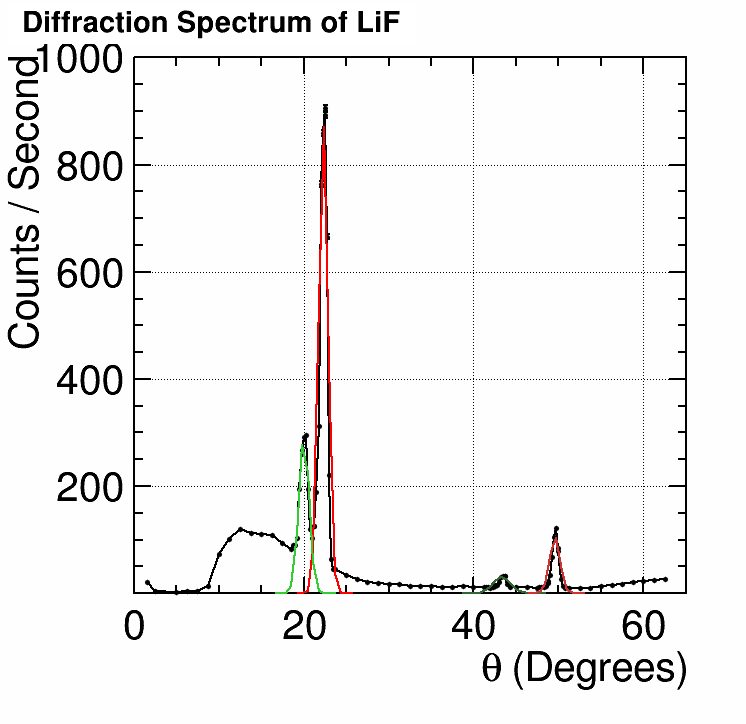
\includegraphics[width=8cm]{Diffraction_LiF.png}
	\caption{Angular diffraction of Lithium Fluoride. Here, $\theta$ refers to the angle of the crystal, so the overall angular displacement of the detector is $2 \theta$.}
	\label{fig:LiF}
\end{figure}

\begin{figure}[H]
	\centering
	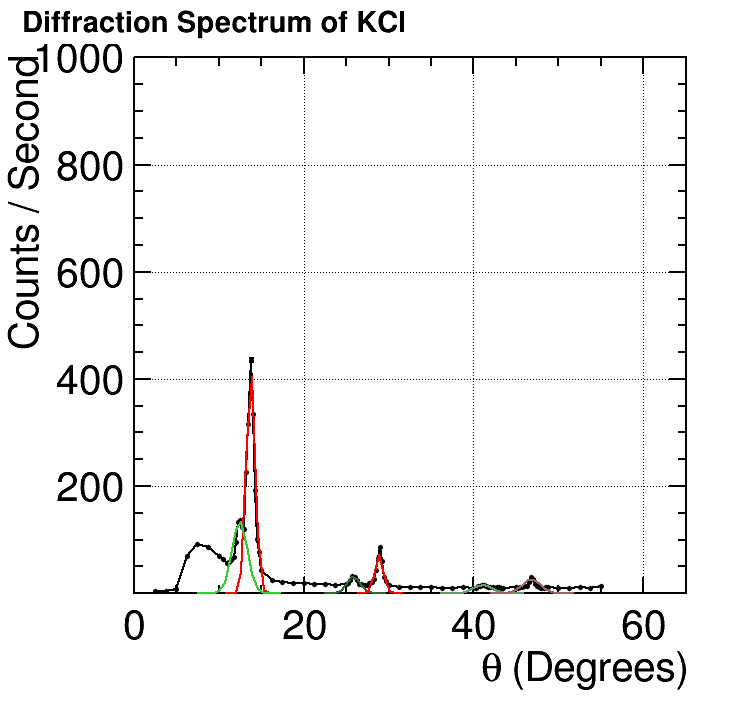
\includegraphics[width=8cm]{Diffraction_KCl.png}
	\caption{Angular diffraction of Potassium Chloride. Here, $\theta$ refers to the angle of the crystal, so the overall angular displacement of the detector is $2 \theta$.}
	\label{fig:KCl}
\end{figure}

From this, we observe two key features. We first can see that there is a bremsstrahlung spectrum which underlays all other features, starting at $\approx10^\circ$ and extending out to the edge of the graph. At the far end ($\theta > 55^\circ$), we enter into a region where x-rays from the source start to enter the detector without scattering off of the crystal (simply due to positioning). This causes these points to be artificially higher than the bremsstrahlung background would otherwise have them. The second feature is the sets of two peaks beginning shortly after the bremsstrahlung spectrum. These are the characteristic x-rays of the source's anode, composed of Copper, scattering off of the crystal structure of the sample according to Bragg's Law, with $n = 1,~2,~3,...$ and an as yet unknown lattice spacing. 
\begin{gather}\label{eq:bragg}
	2d\sin{\theta} = n \lambda
\end{gather}
Using the data gathered above, in concert with the known $K_\alpha$ and $K_\beta$ values, we can determine the experimental values for the lattice spacing:
\begin{gather}
	2d\sin{\theta} = n\lambda \rightarrow d = \frac{n\lambda}{d\sin{\theta}} \nonumber \\
	\downarrow E_\gamma = \frac{hc}{\lambda} \rightarrow \lambda = \frac{hc}{E} \nonumber \\
	d = \frac{n (hc/E)}{2 \sin{\theta}} = \frac{nhc}{2E\sin{\theta}}
\end{gather}
The known energy values for copper are:
\begin{gather}
	K_\alpha = 8037.8 ~eV \nonumber \\
	K_\beta = 8905.29 ~eV \nonumber
\end{gather}
The value of $\theta$ was determined by using a gaussian fit combined with a polynomial background, which we calculated using ROOT. From the parameters of this fit, we can extract $\theta \pm \delta \theta$. Thus we construct the following table for LiF:
\begin{table}[htbp]
	\begin{center}
	\begin{tabular}{|r|r|r|r|r|r|l|}
		\hline
		n & $\theta$ (Deg) & $\delta \theta$ (Deg) & $K$ &  $d$ (nm) & \multicolumn{1}{r|}{$\delta d$ (nm)} \\ \hline
		1 & 20.0293 & 0.61075 & $\beta$ &  0.2034 & 0.005947 \\ \hline
		1 & 22.3206 & 0.55230 & $\alpha$ &  0.2032 & 0.004771 \\ \hline
		2 & 43.3667 & 1.01729 & $\beta$ &  0.2029 & 0.003814 \\ \hline
		2 & 49.5563 & 0.59909 & $\alpha$ &  0.2028 & 0.001808 \\ \hline
	\end{tabular}
	\end{center}
	\caption{Calculated lattice spacing for LiF}
	\label{table:LiF}
\end{table}
Using this method, and averaging the results, we obtain an average value for the lattice spacing for all three crystals:
\begin{table}[htbp]
	\begin{center}
	\begin{tabular}{|l|r|r|}
		\hline
		Crystal & \multicolumn{1}{l|}{$d_{avg}$ (nm)} & \multicolumn{1}{l|}{$\delta d_{avg}$ (nm)} \\ \hline
		LiF & 0.2031 & 0.002179 \\ \hline
		Kcl & 0.3199 & 0.007197 \\ \hline
		NaCl & 0.2875 & 0.004851 \\ \hline
	\end{tabular}
	\end{center}
	\caption{Average value for the lattice spacing for all three crystals}
	\label{table:d_average}
\end{table}
We will compare these values to their known values in the coming sections.

\section{Theoretical Model}

\subsection{X-Ray Florescence}

\subsection{X-Ray Diffraction}

\begin{figure}[H]
	\centering
	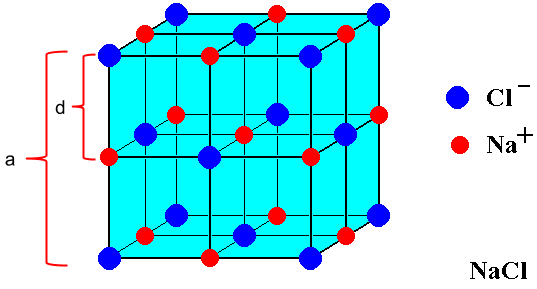
\includegraphics[width=5cm]{nacl_lattice.png}
	\caption{Structure of NaCl, a face centered cubic crystal.}
	\label{fig:lattice_nacl}
\end{figure}

\section{Comparison of Theory and Experiment}

\subsection{X-Ray Florescence}

\subsection{X-Ray Diffraction}

\section{Discussion}

\section{Author Contributions}

\begin{thebibliography}{6}
	
	\bibitem{milissinos}
	A.C. Melissinos, Experiments in Modern Physics (Academic Press, NY, 1966).
	
	\bibitem{bevington}
	Philip R. Bevington and D. Keith Robinson, Data Reduction and Error Analysis 3rd edition (McGraw-Hill, 2003).
	
	\bibitem{eisberg}
	R. M. Eisberg et al., Chapter 14: X-Rays. Fundamentals of Modern Physics,  (Wiley, 1961), Physics Library Ref. QC173.E38.

	\bibitem{frenchtable}
	Laboratoire National Henri Becquerel. Table de Radionucléides (2015) \url{http://www.nucleide.org/DDEP_WG/Nuclides/Cs-137_tables.pdf}
	
	\bibitem{xrd_report}
	Mihaly, Laszlo and PMK. X-Ray Diffraction. (Stony Brook University, 2001)


\end{thebibliography}

\begin{appendix}

\section{Validation of the $\chi^2$ Minimization in ROOT} \label{section:root}
For this experiment, we used ROOT, a c++ based data analysis software, to plot and fit functions to our data. To verify that ROOT calculates a correct value for $\chi^{2}$, we performed a hand calculation cross check with a simple set of data. The data set we used for this cross check was $\{ (11.0 \pm 0.0, 23.0 \pm 0.5), (14.0 \pm 0.0, 25.0 \pm 0.5), (20.0 \pm 0.0, 35.0 \pm 0.5), (25.0 \pm 0.0, 39.0 \pm 0.5) \}$. We plotted this data and fit it to a linear function $f(x) = [0] + [1]*x$. This plot is shown in Fig.~\ref{Fig:rootproof}.
\begin{figure}[H]
	\centering
	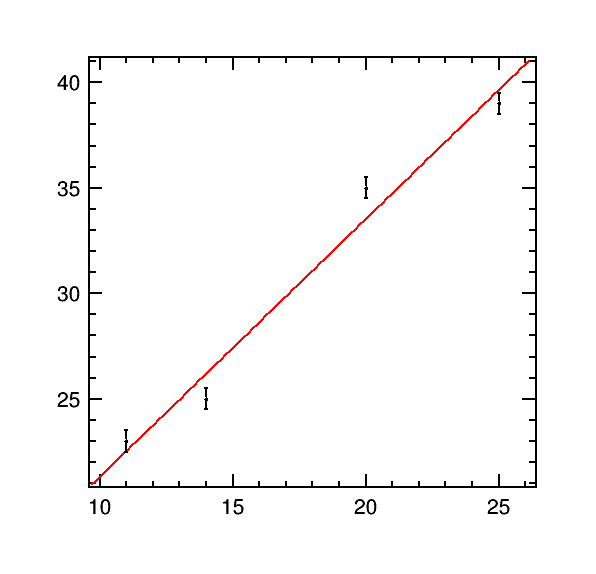
\includegraphics[width=0.4\textwidth]{rootproof.png}
	\caption{Sample Data Fitted to a Line}
	\label{Fig:rootproof}
\end{figure}
The function obtained from this fit was $f(x) = 9.11111 + 1.22222x$ with a chi-squared of $\chi ^{2} = 16.8889$. We then performed a hand calculation of the $\chi ^{2}$ using Eq.~\ref{eq:chisq}.
\begin{gather}\label{eq:chisq}
\chi ^{2} = \sum \frac{(f(x_i) - y_i)^{2}}{\sigma_i^2}
\end{gather}
When performing this hand calculation we also obtained a value of $\chi ^{2} = 16.8889$, verifying ROOT's ability to calculate $\chi ^{2}$.
\begin{align*}
\chi ^{2} =& \frac{(f(11.0) - 23.0)^{2}}{(0.5)^2} + \frac{(f(14.0) - 25.0)^{2}}{(0.5)^2} \\
&+ \frac{(f(20.0) - 35.0)^2}{(0.5)^2} + \frac{(f(25.0) - 39.0)^{2}}{(0.5)^2} \\
&= 16.8889
\end{align*}

\section{Analysis Code} \label{section:analysis_code}
All of the analysis code used for this lab can be found in the following git repository: 
\begin{verbatim}
https://github.com/jlabounty/SeniorLab/tree
/master/XRF_XRD
\end{verbatim}

\end{appendix}

\end{document}